
\documentclass[compress]{beamer}

\mode<presentation> {

\usetheme{Berlin}
\usecolortheme{seahorse}
\useoutertheme[subsection=false]{smoothbars} 


\setbeamertemplate{navigation symbols}{} 
}
\usepackage{graphicx} 
\usepackage{booktabs}
\usepackage{amssymb} 

%----------------------------------------------------------------------------------------
%	TITLE PAGE
%----------------------------------------------------------------------------------------

\title{Introduction to Markov Chain Monte Carlo}

\author{Helen Johnson}
\date{8th July 2014}

\begin{document}

\begin{frame}
\titlepage
\end{frame}

\section{Introduction}
\label{sec-5}
\begin{frame}[label=sec-5-1]{Recap. on Bayesian inference}
This morning we saw that the posterior distribution of $\theta$, given observed data is

$$ p(\theta | data) \propto p(data |\theta) p(\theta)$$\\~\\

Our aims are to:
\begin{itemize}
\item explore this distribution
\item draw samples from it
\end{itemize}
\end{frame}

\section{Rejection sampling}
\label{sec-6}
\begin{frame}[label=sec-5-2]{Rejection sampling}
\begin{columns}[c] 
\column{.5\textwidth} 
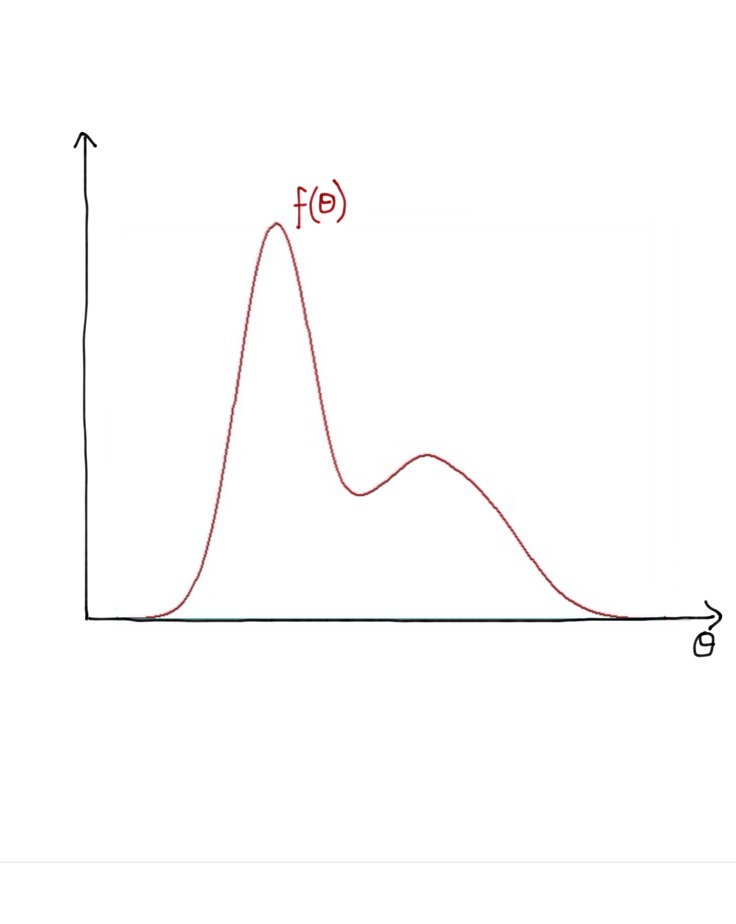
\includegraphics[width=.8\linewidth]{RS1.png}

\column{.5\textwidth}
Consider a distribution $f(\theta)$ which:
\begin{itemize}
\item is possible to evaluate
\item is difficult to sample from
\end{itemize}
\end{columns}
\end{frame}

\begin{frame}[label=sec-5-3]{Rejection sampling}
\begin{columns}[c] 
\column{.5\textwidth} 
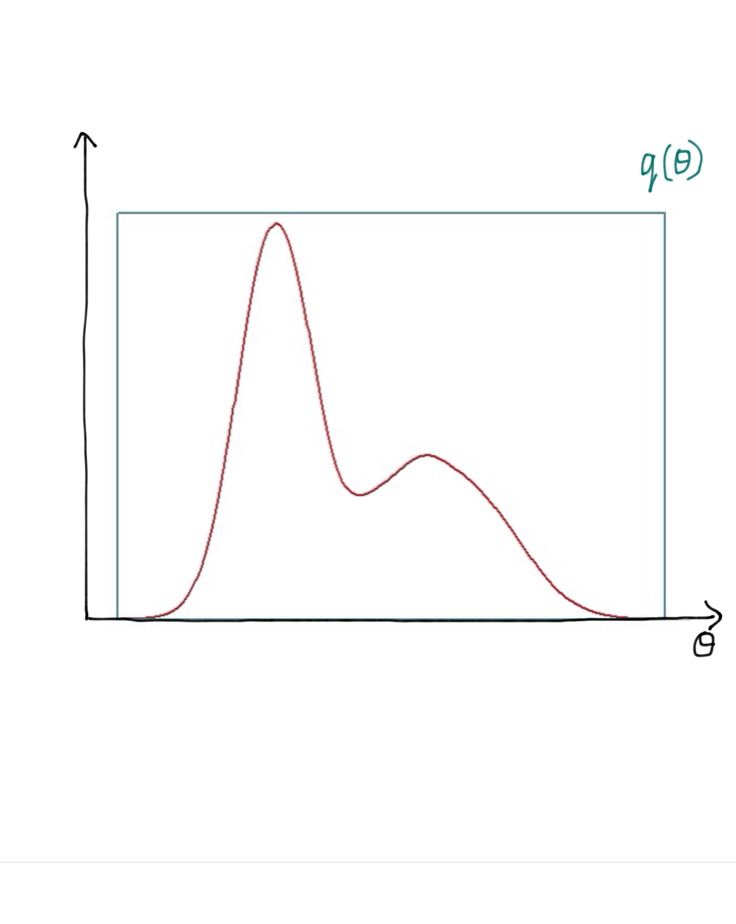
\includegraphics[width=.8\linewidth]{RS2.png}

\column{.5\textwidth}
Consider a distribution $f(\theta)$ which:
\begin{itemize}
\item is possible to evaluate
\item is difficult to sample from
\end{itemize}
Rejection sampling uses a \alert{proposal distribution $q(\theta)$} which:
\begin{itemize}
\item is possible to evaluate
\item is easy to sample from
\item has a greater density than $f(\theta)$ for all $\theta$
\end{itemize}
\end{columns}
\end{frame}

\begin{frame}[label=sec-5-4]{Rejection sampling}
\begin{columns}[c] 
\column{.5\textwidth} 
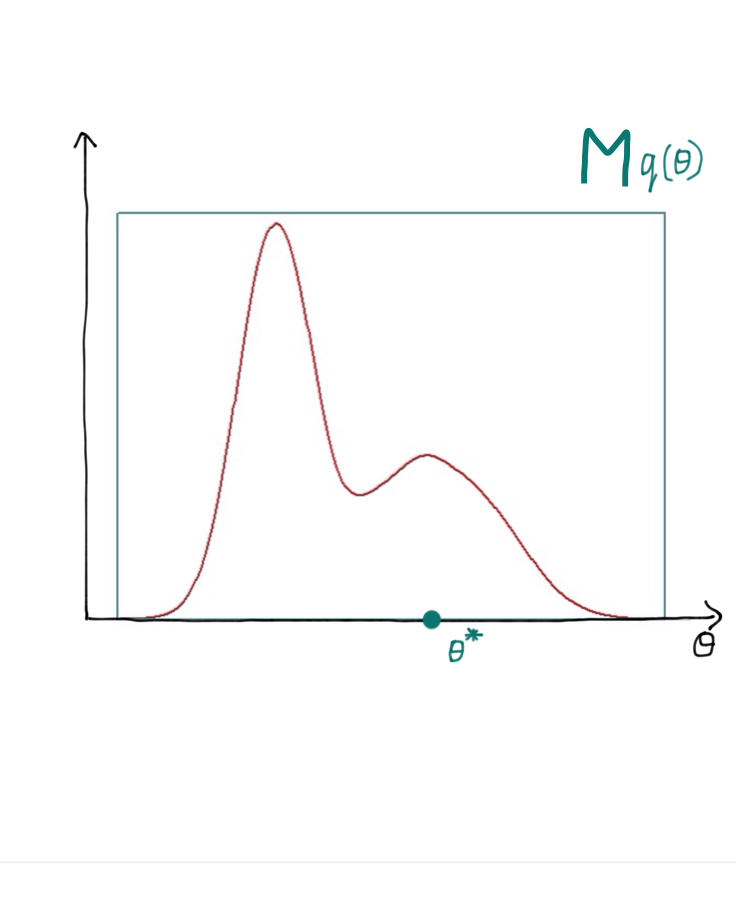
\includegraphics[width=.8\linewidth]{RS3.png}

\column{.5\textwidth}
The algorithm proceeds as follows:\\
\begin{itemize}
\item Sample $\theta^*$ from $q(\theta)$
\end{itemize}
\end{columns}
\end{frame}

\begin{frame}[label=sec-5-5]{Rejection sampling}
\begin{columns}[c] 
\column{.5\textwidth} 
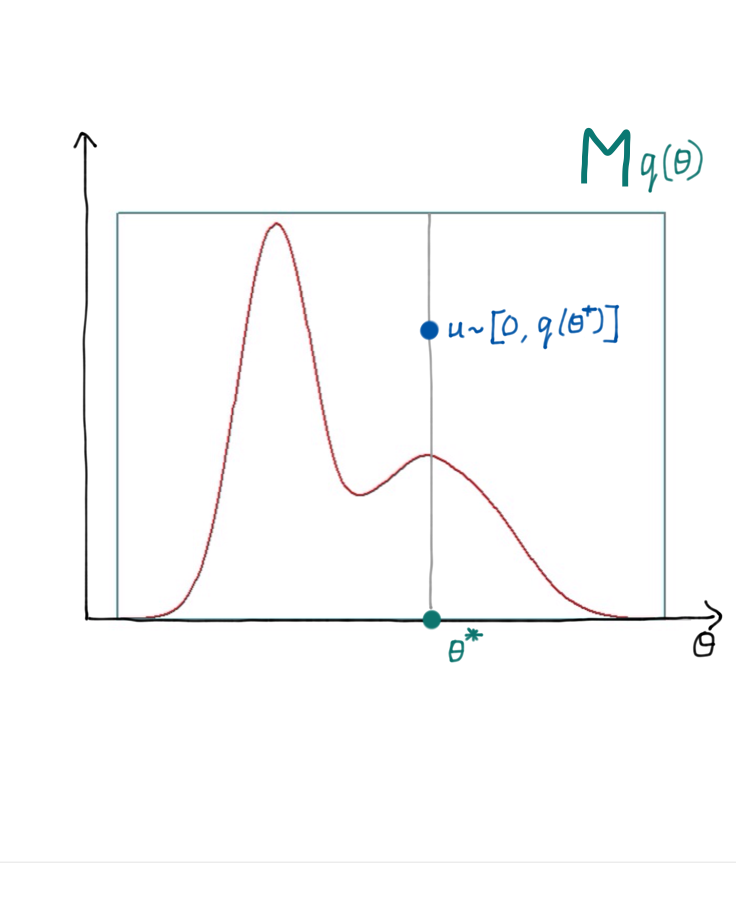
\includegraphics[width=.8\linewidth]{RS4.png}

\column{.5\textwidth}
The algorithm proceeds as follows:\\
\begin{itemize}
\item Sample $\theta^*$ from $q(\theta)$
\item Draw a random number $u ~ Uni[0, q(\theta^*)]$
\end{itemize}
\end{columns}
\end{frame}

\begin{frame}[label=sec-5-6]{Rejection sampling}
\begin{columns}[c] 
\column{.5\textwidth} 
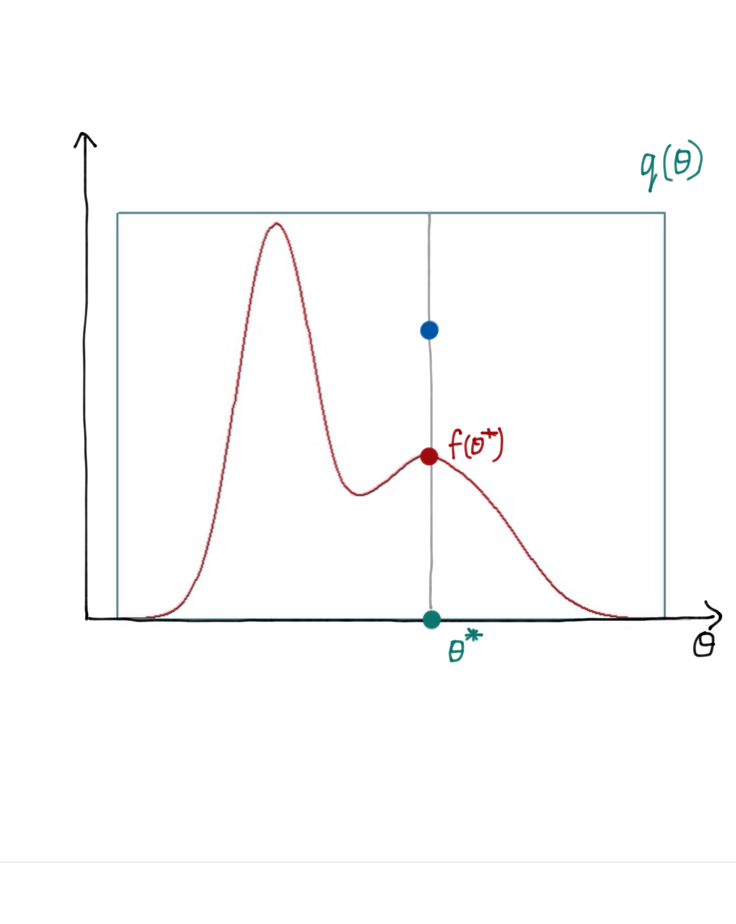
\includegraphics[width=.8\linewidth]{RS5.png}

\column{.5\textwidth}
The algorithm proceeds as follows:\\
\begin{itemize}
\item Sample $\theta^*$ from $q(\theta)$
\item Draw a random number $u ~ Uni[0, q(\theta^*)]$
\item Evaluate $f(\theta^*)$
\end{itemize}
\end{columns}
\end{frame}

\begin{frame}[label=sec-5-7]{Rejection sampling}
\begin{columns}[c] 
\column{.5\textwidth} 
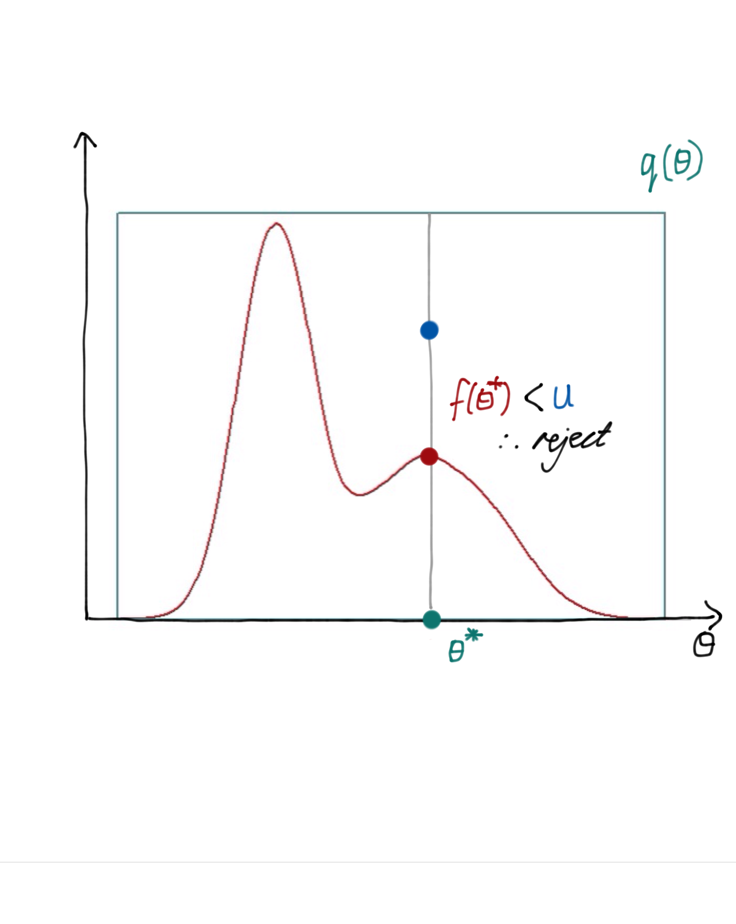
\includegraphics[width=.8\linewidth]{RS6.png}

\column{.5\textwidth}
The algorithm proceeds as follows:\\
\begin{itemize}
\item Sample $\theta^*$ from $q(\theta)$
\item Draw a random number $u ~ Uni[0, q(\theta^*)]$
\item Evaluate $f(\theta^*)$
\item If $f(\theta^*) > u accept, else reject$
\end{itemize}
\end{columns}
\end{frame}

\begin{frame}[label=sec-5-8]{Rejection sampling}
\begin{columns}[c] 
\column{.5\textwidth} 
\only<1>{\href{RS7.png}{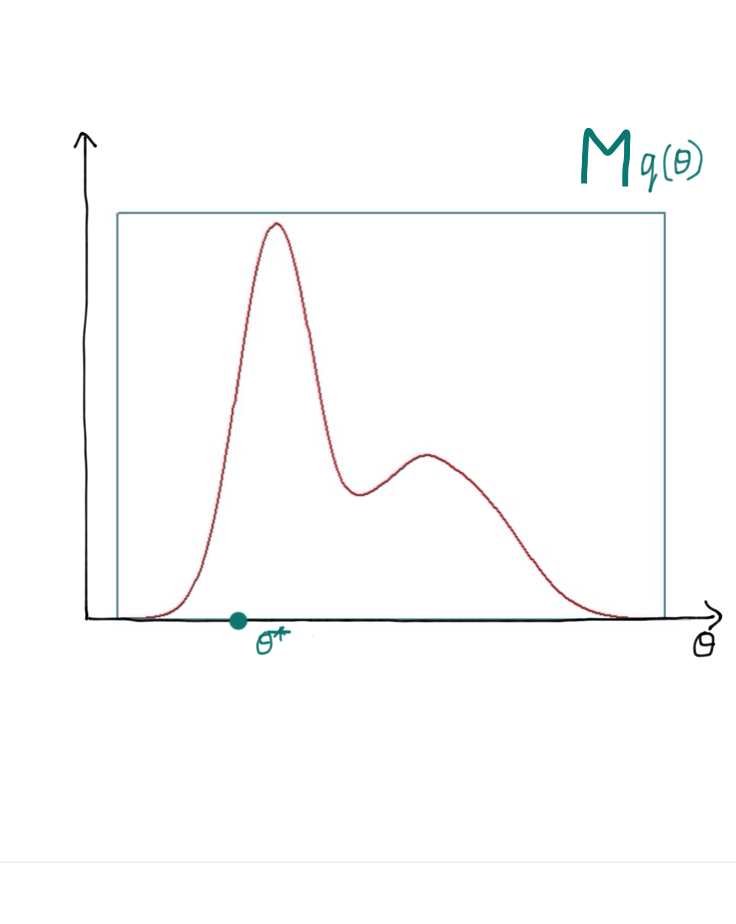
\includegraphics[width=.8\linewidth]{RS7.png}}}
\only<2>{\href{RS8.png}{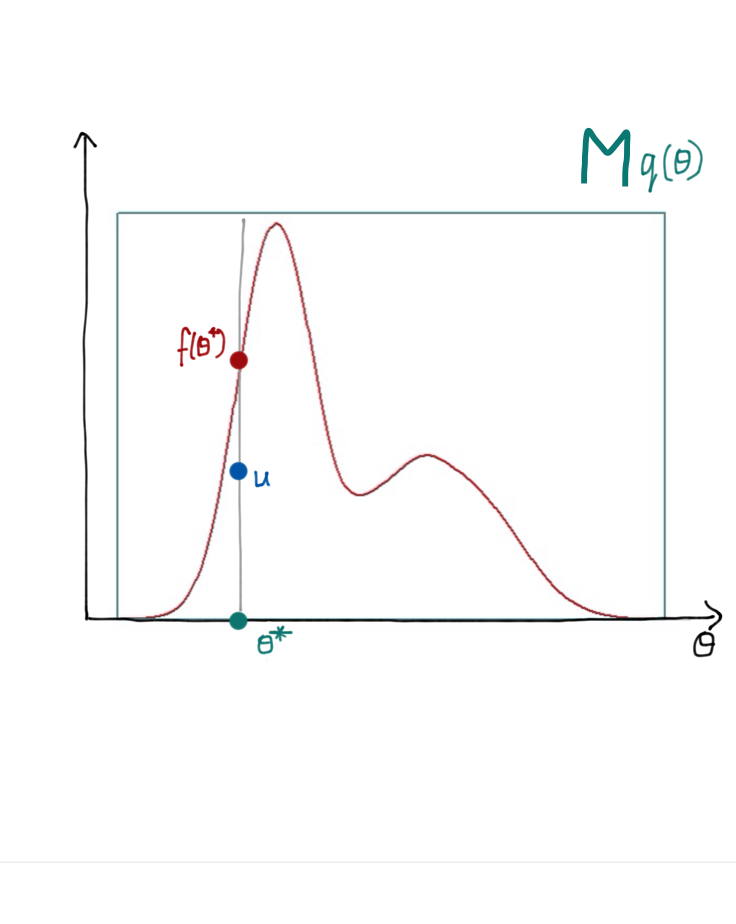
\includegraphics[width=.8\linewidth]{RS8.png}}}
\only<3>{\href{RS9.png}{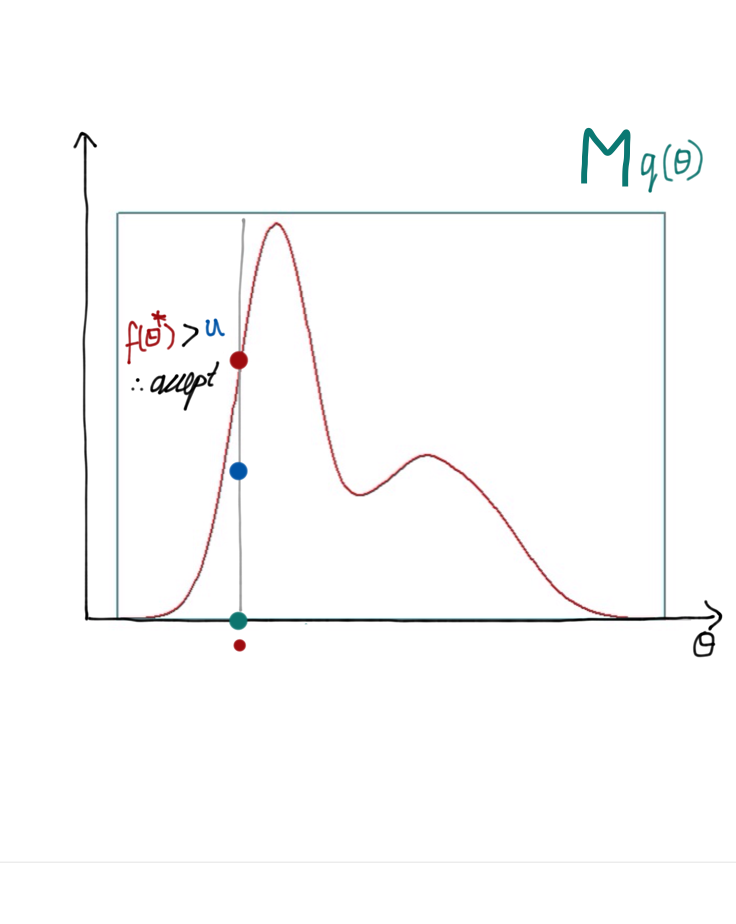
\includegraphics[width=.8\linewidth]{RS9.png}}}
\only<4>{\href{RS10.png}{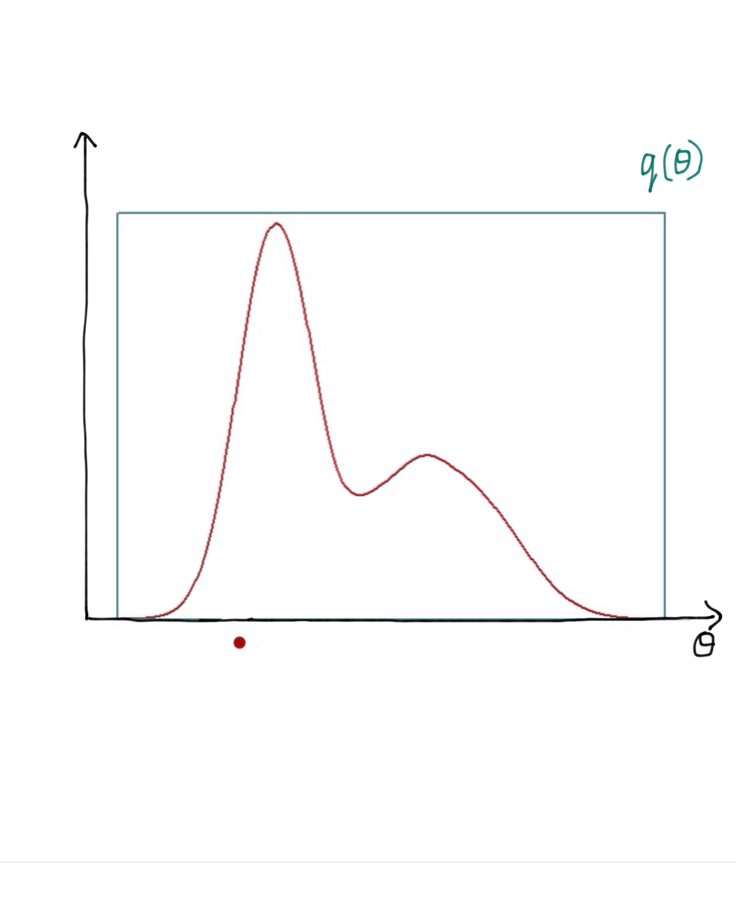
\includegraphics[width=.8\linewidth]{RS10.png}}}
\only<5>{\href{RS11.png}{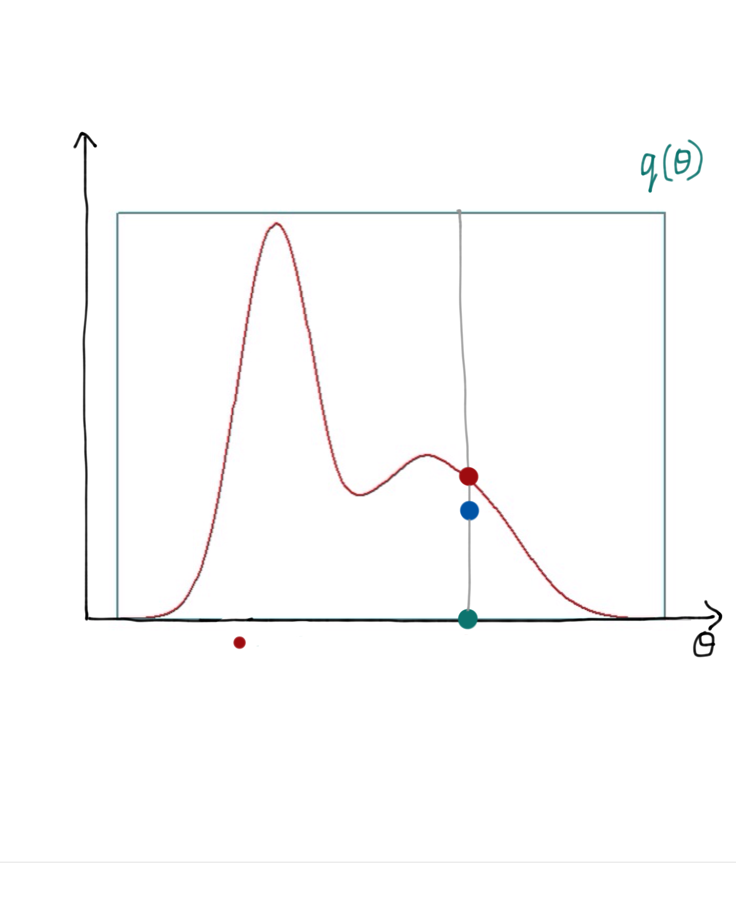
\includegraphics[width=.8\linewidth]{RS11.png}}}
\only<6>{\href{RS12.png}{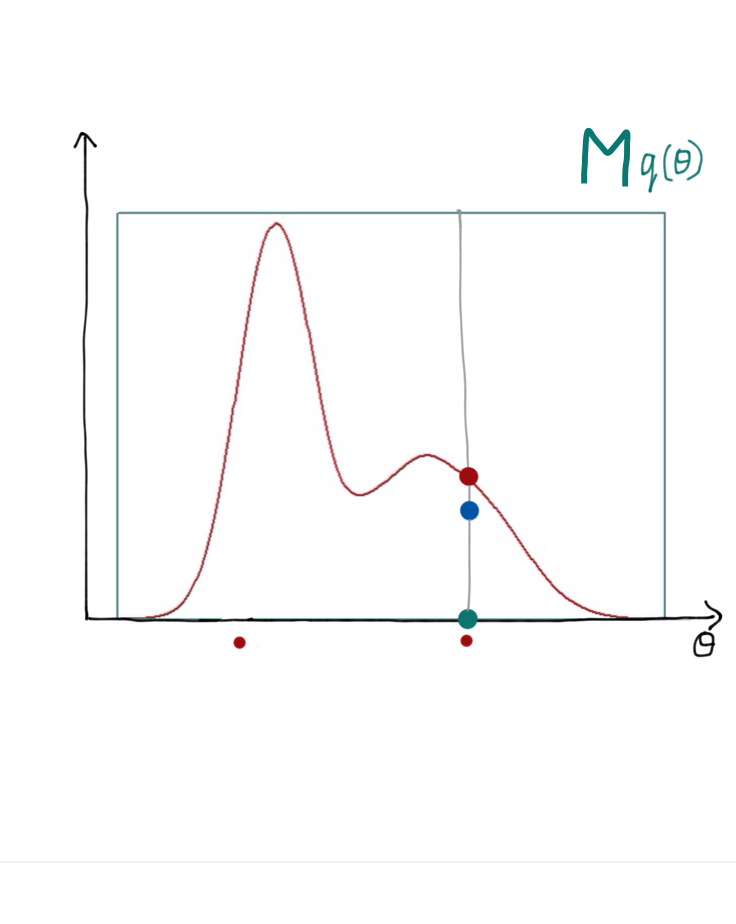
\includegraphics[width=.8\linewidth]{RS12.png}}}
\only<7>{\href{RS13.png}{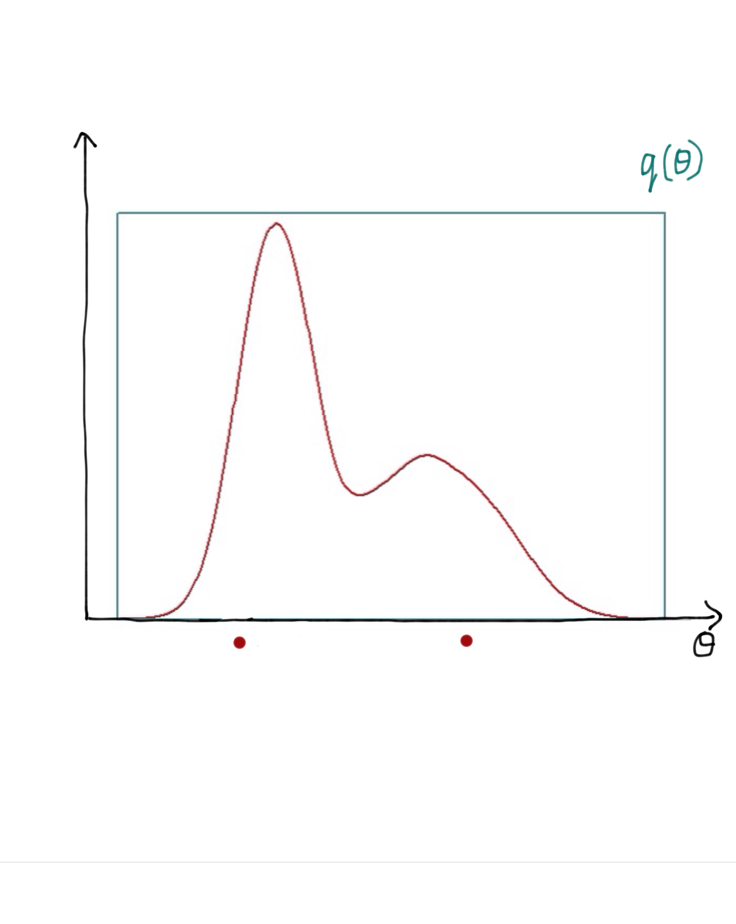
\includegraphics[width=.8\linewidth]{RS13.png}}}
\only<8>{\href{RS14.png}{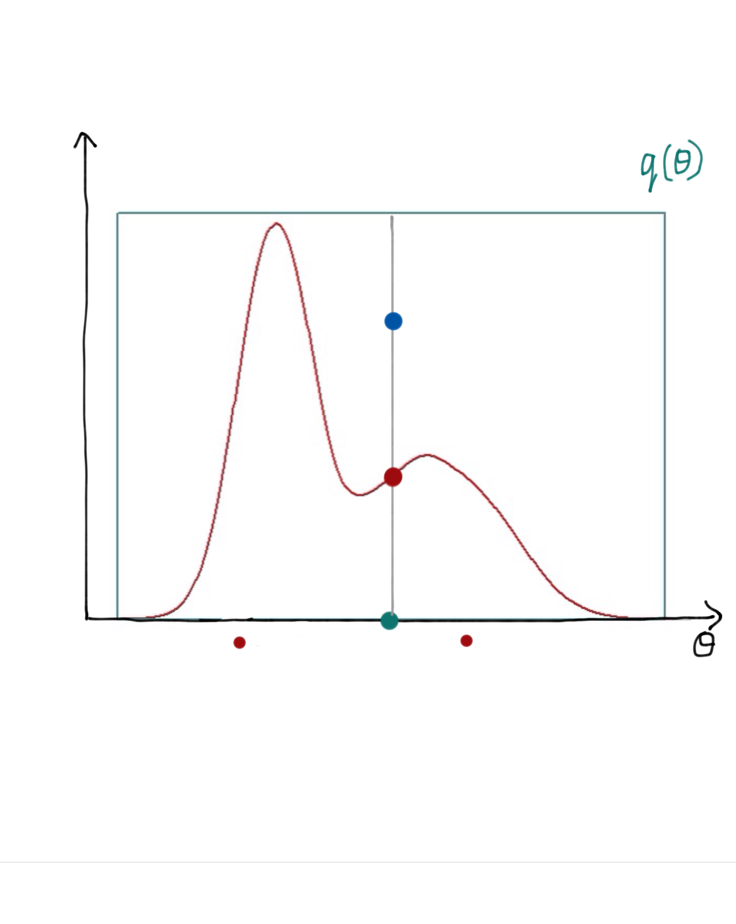
\includegraphics[width=.8\linewidth]{RS14.png}}}
\only<9>{\href{RS15.png}{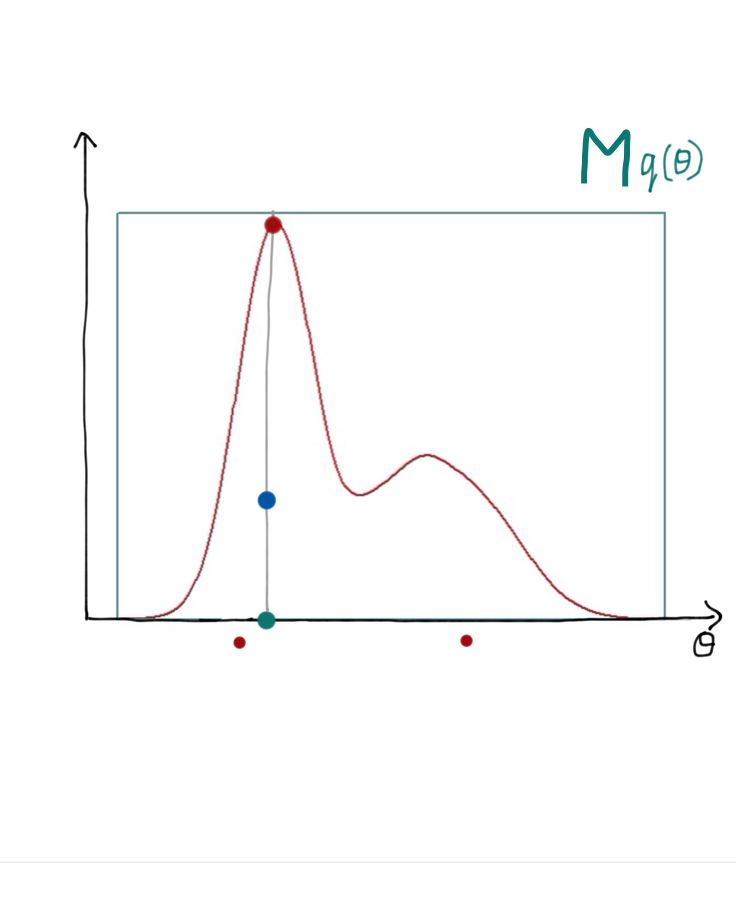
\includegraphics[width=.8\linewidth]{RS15.png}}}
\only<10>{\href{RS16.png}{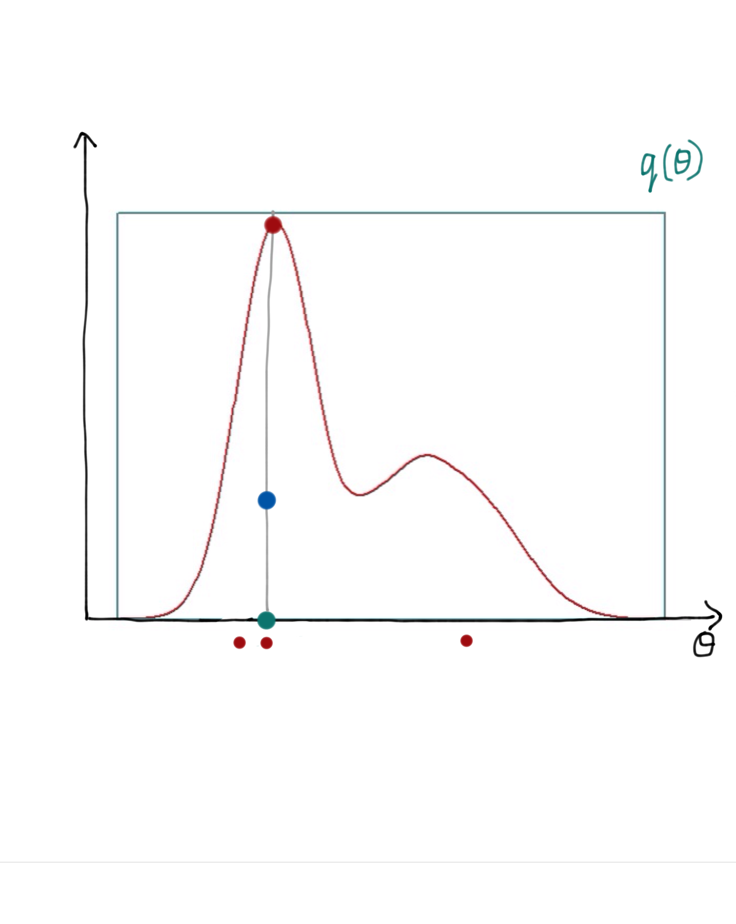
\includegraphics[width=.8\linewidth]{RS16.png}}}
\only<11>{\href{RS17.png}{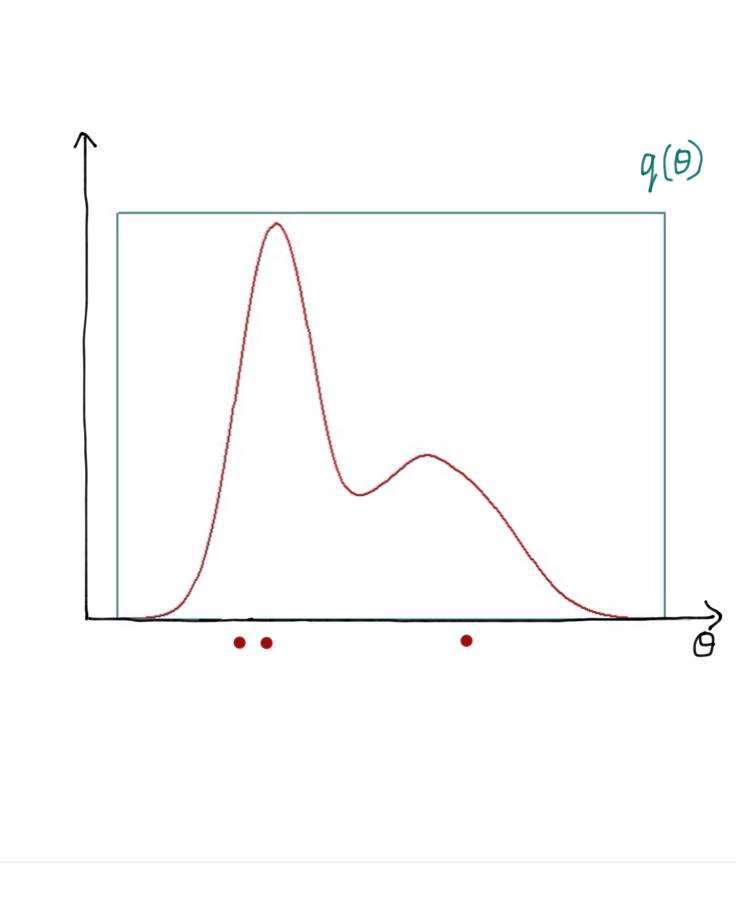
\includegraphics[width=.8\linewidth]{RS17.png}}}
\only<12>{\href{RS18.png}{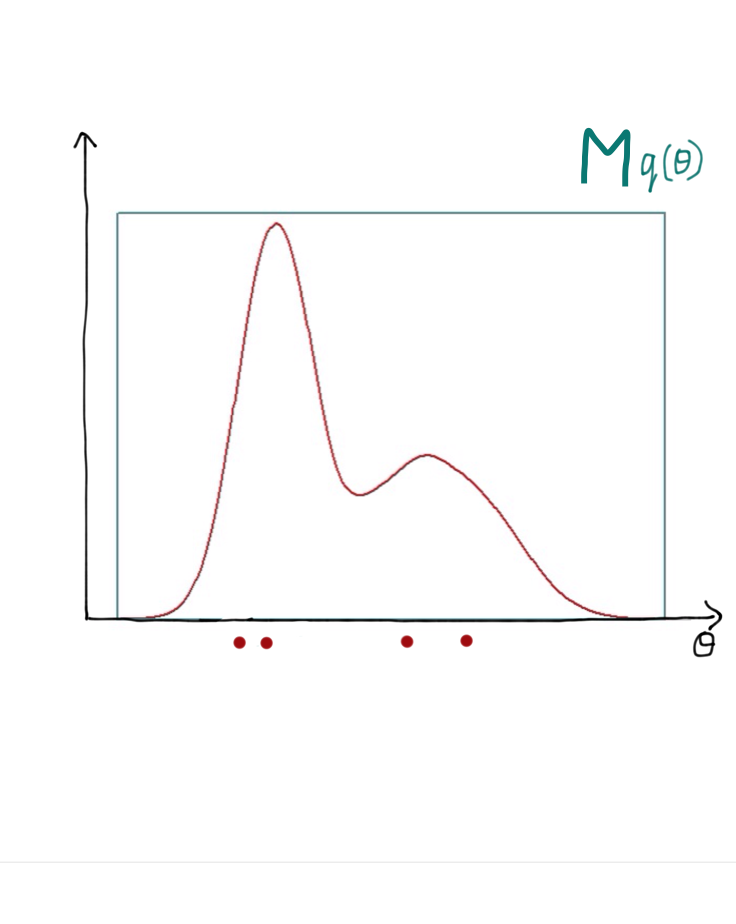
\includegraphics[width=.8\linewidth]{RS18.png}}}
\only<13>{\href{RS19.png}{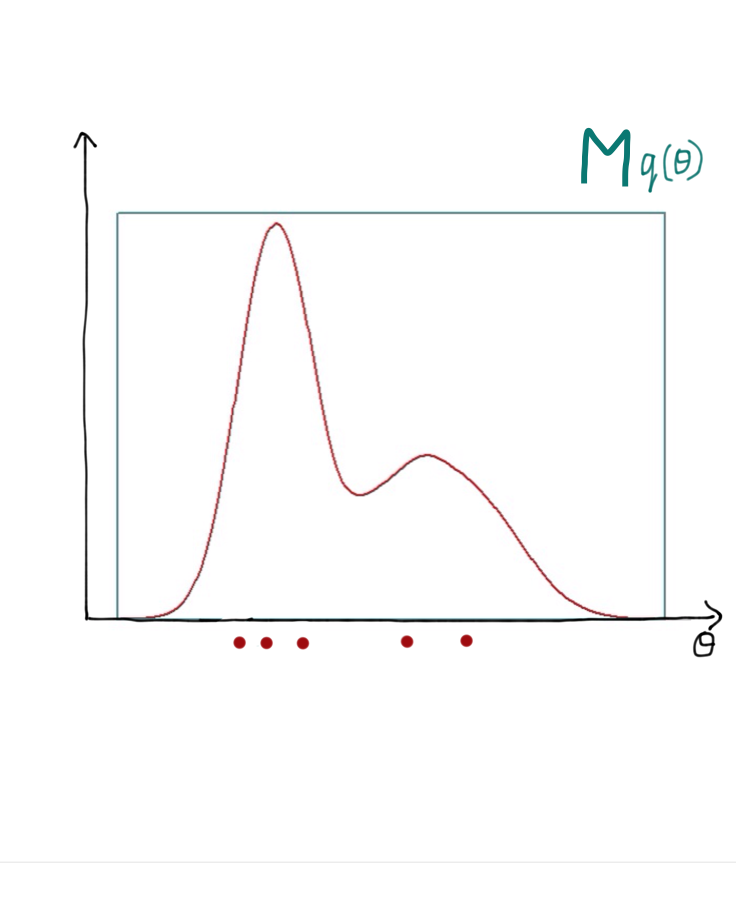
\includegraphics[width=.8\linewidth]{RS19.png}}}
\only<14>{\href{RS20.png}{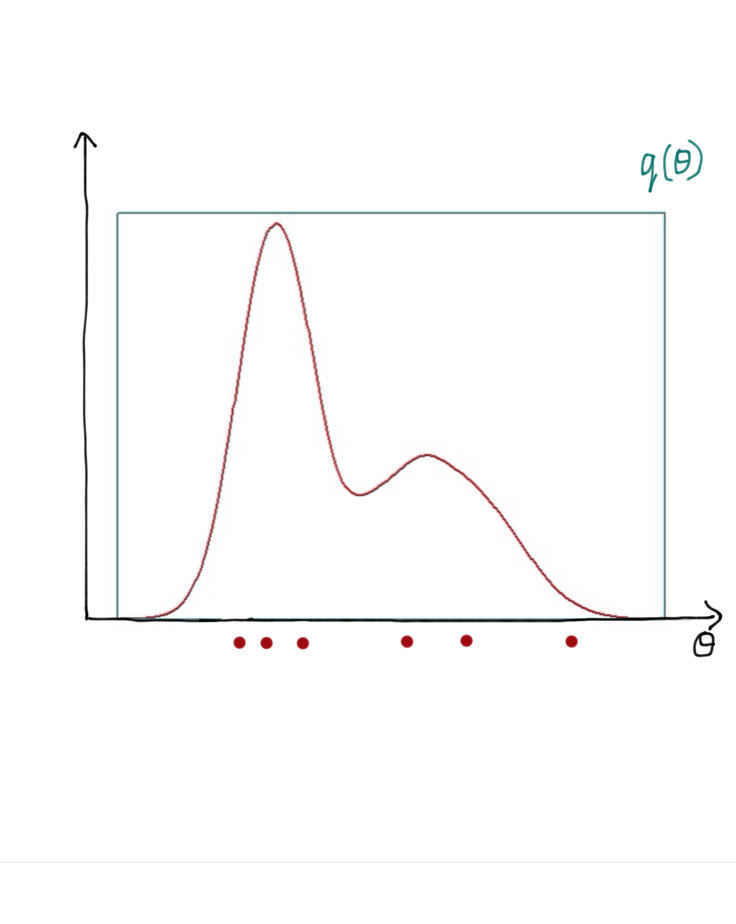
\includegraphics[width=.8\linewidth]{RS20.png}}}
\only<15>{\href{RS21.png}{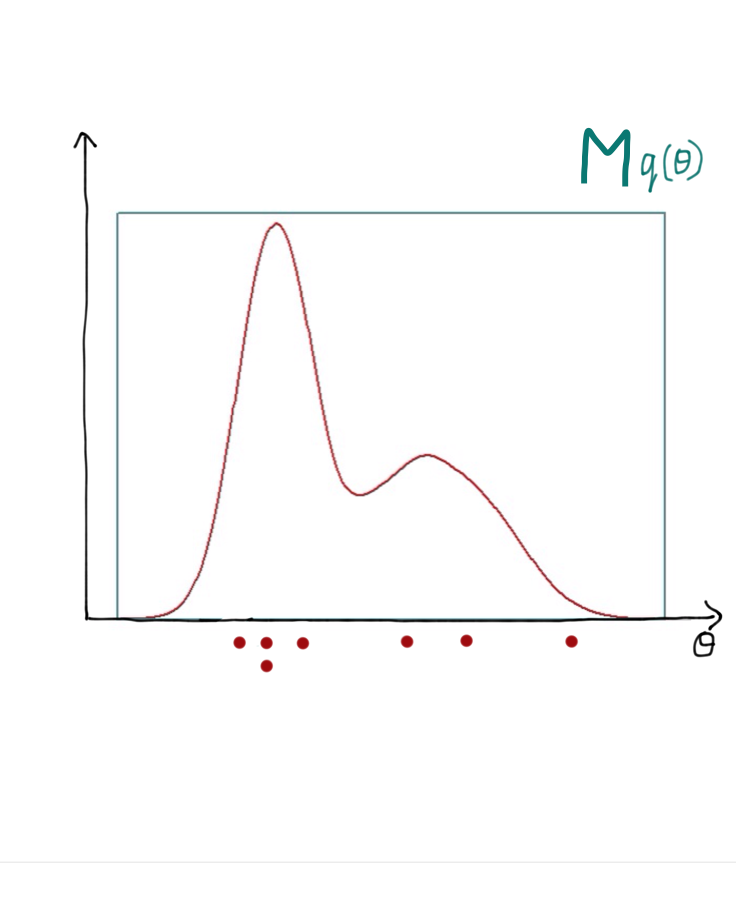
\includegraphics[width=.8\linewidth]{RS21.png}}}
\only<16>{\href{RS22.png}{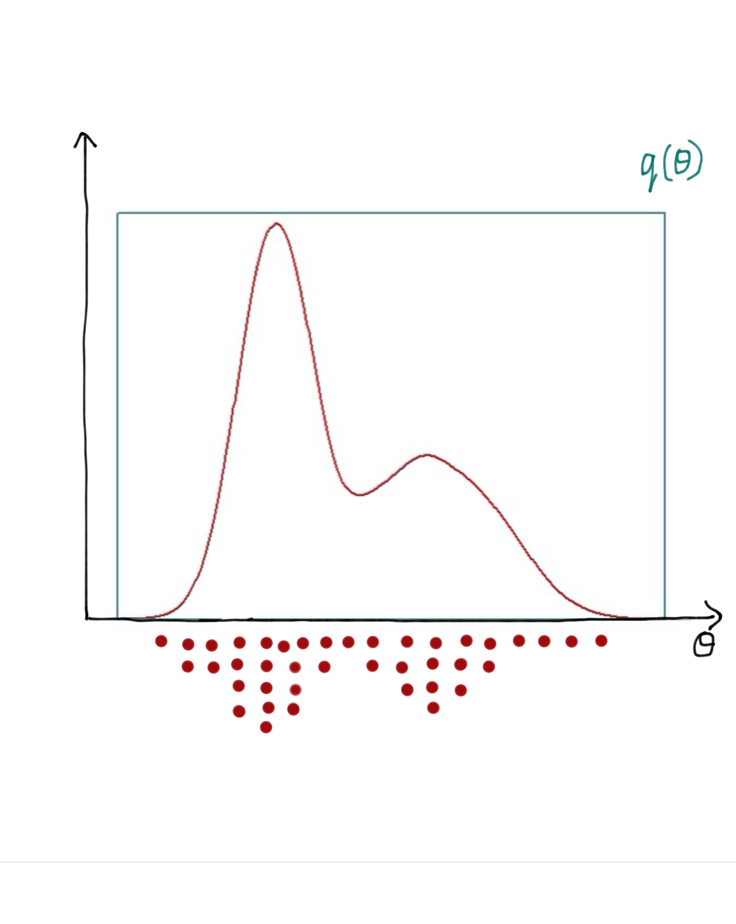
\includegraphics[width=.8\linewidth]{RS22.png}}}

\column{.5\textwidth}
The algorithm proceeds as follows:\\
\begin{itemize}
\item Sample $\theta^*$ from $q(\theta)$
\item Draw a random number $u ~ Uni[0, q(\theta^*)]$
\item Evaluate $f(\theta^*)$
\item If $f(\theta^*) > u accept, else reject$
\item Repeat
\end{itemize}
\end{columns}
\end{frame}

\begin{frame}[label=sec-5-9]{Rejection sampling}
\begin{columns}[c] 
\column{.5\textwidth}
\begin{itemize}
\item Rejection sampling works best if $q(\theta) \approx f(\theta)$ \\~\\
\item Requiring $q(\theta) \geqslant f(\theta)$ for all $\theta$ can make rejection rate v. high\\~\\
\item Even more limited in high dimensions
\end{itemize}

\column{.5\textwidth}
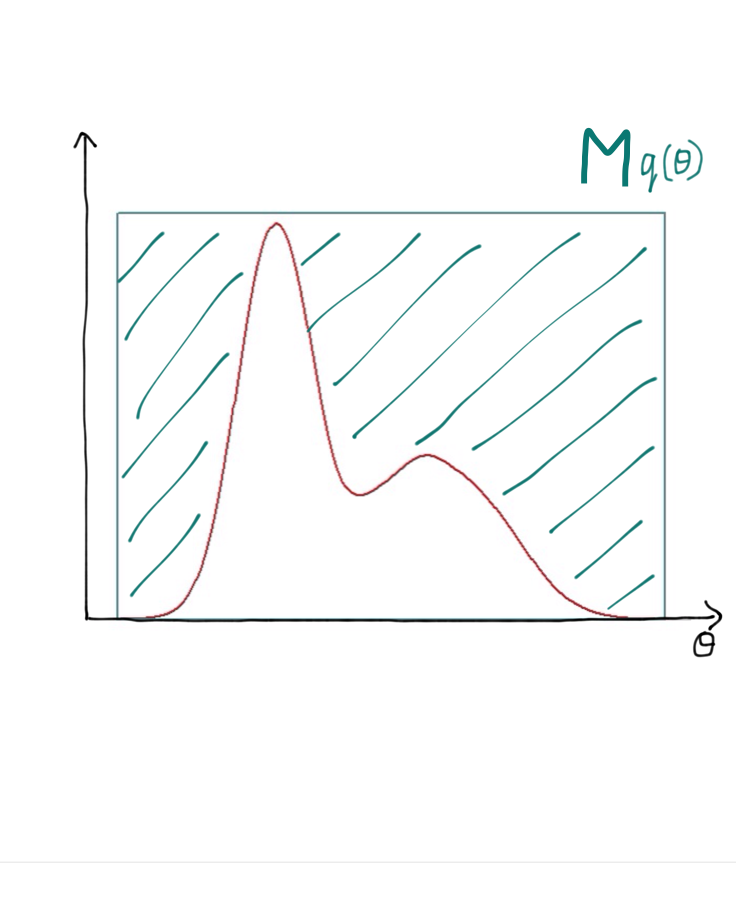
\includegraphics[width=.8\linewidth]{RS23.png}
\end{columns}
\end{frame}


\section{What is Markov Chain Monte Carlo?}
\label{sec-7}
\begin{frame}[label=sec-7-1]{Markov Chain Monte Carlo}
\begin{itemize}
\item In Markov Chain Monte Carlo (MCMC) we do not define one proposal density $q(\theta) \geqslant f(\theta)$.\\~\\
\item Rather we build up a \alert{chain} of samples where each proposed $\theta^*$ depends on the previous one.\\~\\
\item The proposal density takes the form $q(\theta^* | \theta)$\\~\\
\item A commonly used MCMC algorithm is \alert{Metropolis-Hastings}
\end{itemize}
\end{frame}


\begin{frame}[label=sec-7-2]{Metropolis-Hastings}
\begin{columns}[c] 
\column{.5\textwidth} 
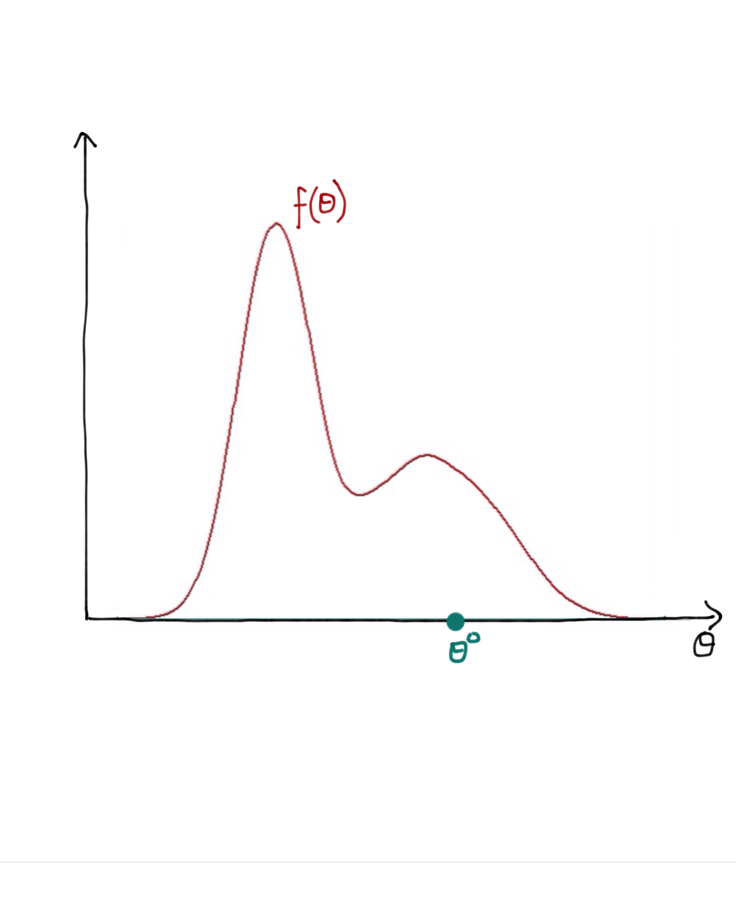
\includegraphics[width=0.8\linewidth]{MH1}

\column{.5\textwidth}
The algorithm proceeds as follows:\\
\begin{itemize}
\item Initialise $\theta^{0}$
\end{itemize}
\end{columns}
\end{frame}


\begin{frame}[label=sec-7-3]{Metropolis-Hastings}
\begin{columns}[c] 
\column{.5\textwidth} 
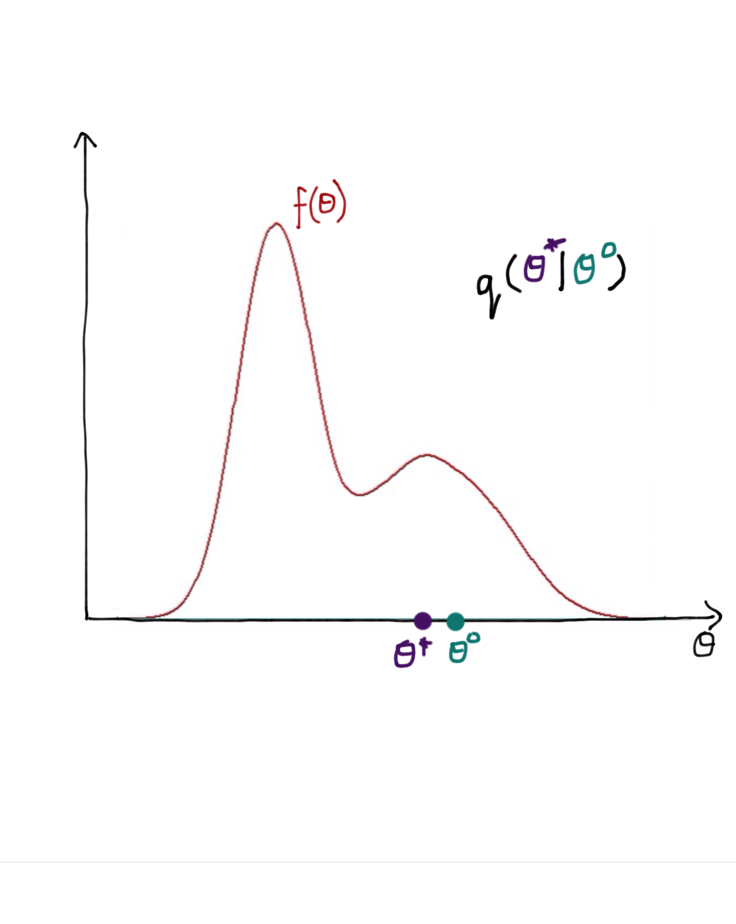
\includegraphics[width=0.8\linewidth]{MH2}

\column{.5\textwidth}
The algorithm proceeds as follows:
\begin{itemize}
\item Initialise $\theta^{0}$
\item Sample $\theta^* \sim q(\theta^*|\theta^{0})$;
\end{itemize}
\end{columns}
\end{frame}


\begin{frame}[label=sec-7-4]{Metropolis-Hastings}
\begin{columns}[c] 
\column{.5\textwidth} 
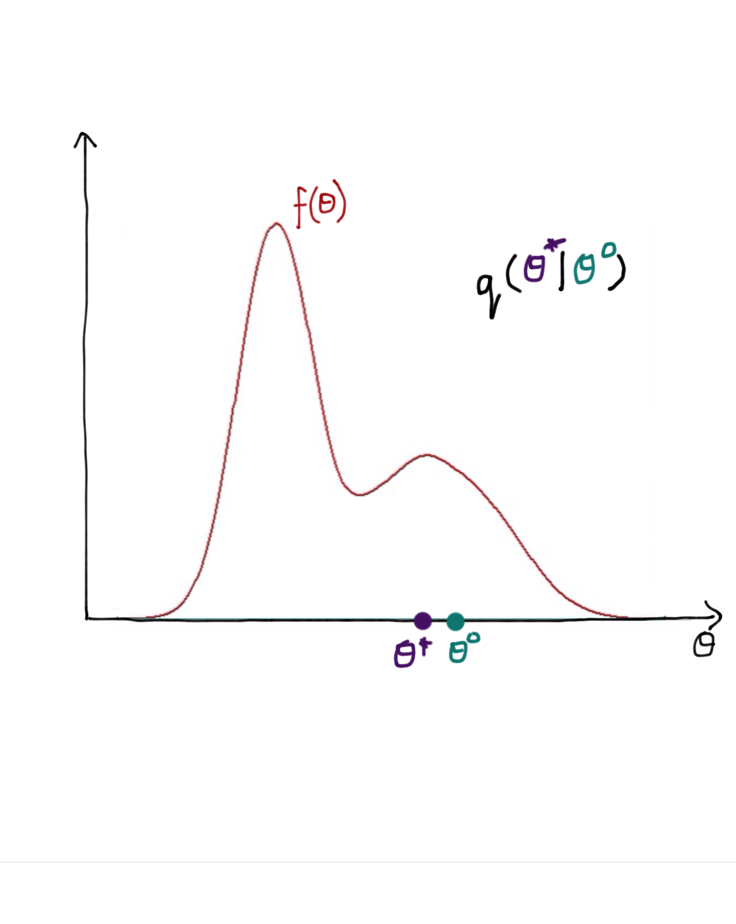
\includegraphics[width=0.8\linewidth]{MH2}

\column{.5\textwidth}
The algorithm proceeds as follows:\\
\begin{itemize}
\item Initialise $\theta^{0}$
\item Sample $\theta^* \sim q(\theta^*|\theta^{0})$
\item Compute acceptance probability, r

\end {itemize}
\end{columns}
\end{frame}

\begin{frame}[label=sec-7-5]{Metropolis-Hastings}
\begin{columns}[c] 
\column{.5\textwidth} 
\begin{block}{Acceptance}
\begin{itemize}
\item If $q(\theta^*|\theta^{0})$ symmetric, then 
$$ r = min(1,\dfrac{f(\theta^*)}{f(\theta)})$$
\end{itemize}
\end{block}

\column{.5\textwidth}
The algorithm proceeds as follows:\\
\begin{itemize}
\item Initialise $\theta^{0}$
\item Sample $\theta^* \sim q(\theta^*|\theta^{0})$
\item Compute acceptance probability, r
\end{itemize}
\end{columns}
\end{frame}

\begin{frame}[label=sec-7-6]{Metropolis-Hastings}
\begin{columns}[c] 
\column{.5\textwidth} 
\begin{block}{Acceptance}
\begin{itemize}
\item If $q(\theta^*|\theta^{0})$ symmetric, then 
$$ r = min(1,\dfrac{f(\theta^*)}{f(\theta)})$$
\item Definitely move to $\theta^*$ if more probable than $\theta$ 
\end{itemize}
\end{block}

\column{.5\textwidth}
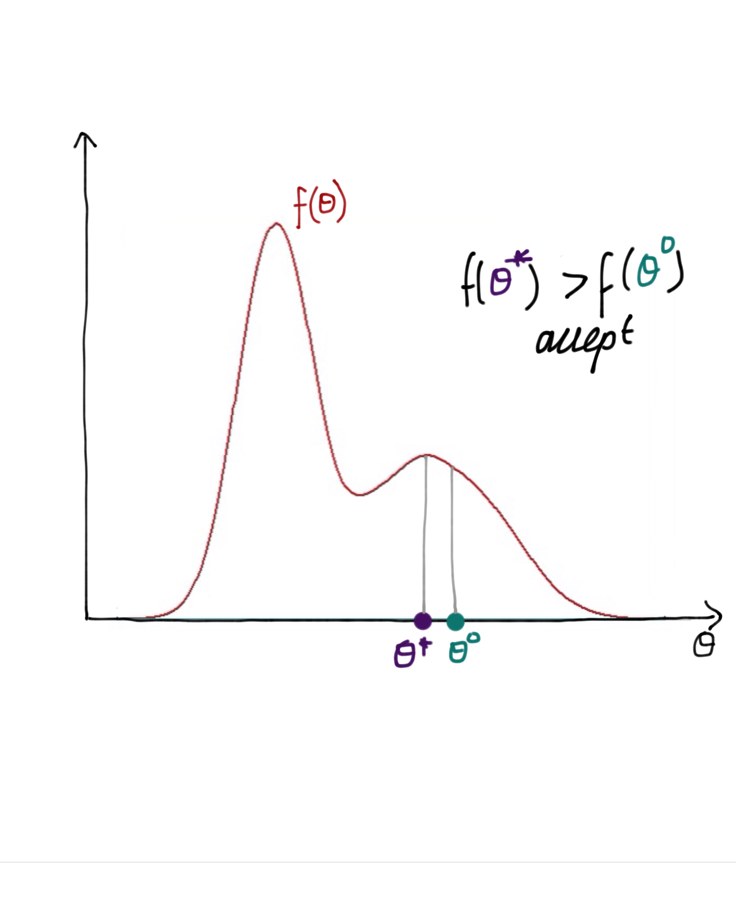
\includegraphics[width=0.8\linewidth]{MH3}
\end{columns}
\end{frame}

\begin{frame}[label=sec-7-7]{Metropolis-Hastings}
\begin{columns}[c] 
\column{.5\textwidth} 
\begin{block}{Acceptance}
\begin{itemize}
\item If $q(\theta^*|\theta^{0})$ symmetric, then 
$$ r = min(1,\dfrac{f(\theta^*)}{f(\theta)})$$
\item Definitely move to $\theta^*$ if more probable than $\theta$ 
\item May move if $\theta^*$ less probable 
\end{itemize}
\end{block}

\column{.5\textwidth}
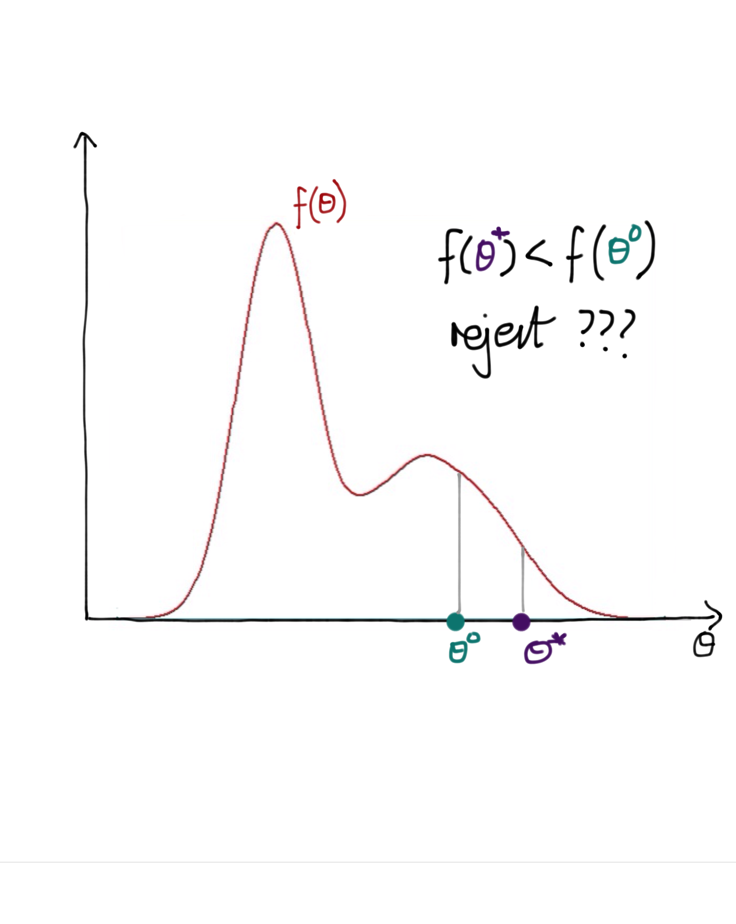
\includegraphics[width=0.8\linewidth]{MH4}
\end{columns}
\end{frame}

\begin{frame}[label=sec-7-8]{Metropolis-Hastings}
\begin{columns}[c] 
\column{.5\textwidth} 
\begin{block}{Acceptance}
\begin{itemize}
\item If $q(\theta^*|\theta^{0})$ symmetric, then 
$$ r = min(1,\dfrac{f(\theta^*)}{f(\theta)})$$
\item Definitely move to $\theta^*$ if more probable than $\theta$ 
\item May move if $\theta^*$ less probable 
\item If asymmetric, make correction: $\dfrac{f(\theta^*)q(\theta|\theta^*)}{f(\theta)q(\theta^*|\theta)}$
\end{itemize}
\end{block}

\column{.5\textwidth}
The algorithm proceeds as follows:\\
\begin{itemize}
\item Initialise $\theta^{0}$
\item Sample $\theta^* \sim q(\theta^*|\theta^{0})$
\item Compute acceptance probability, r
\end{itemize}
\end{columns}
\end{frame}

\begin{frame}[label=sec-7-9]{Metropolis-Hastings}
\begin{columns}[c] 
\column{.5\textwidth} 
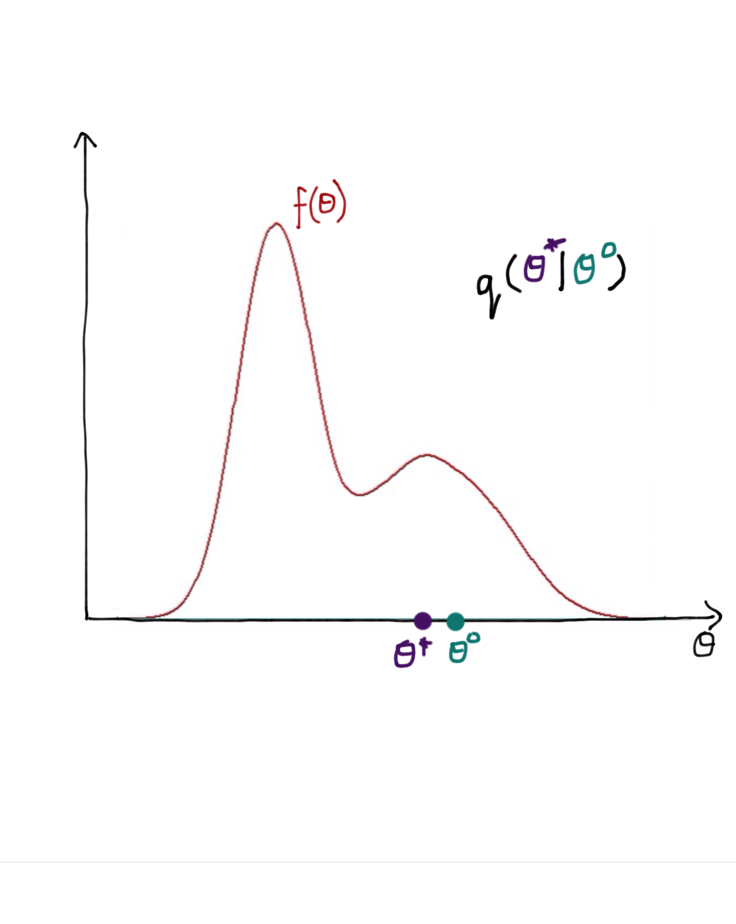
\includegraphics[width=0.8\linewidth]{MH2}

\column{.5\textwidth}
The algorithm proceeds as follows:\\
\begin{itemize}
\item Initialise $\theta^{0}$
\item Sample $\theta^* \sim q(\theta^*|\theta^{0})$
\item Compute acceptance probability, r
\end {itemize}
\end{columns}
\end{frame}

\begin{frame}[label=sec-7-10]{Metropolis-Hastings}
\begin{columns}[c] 
\column{.5\textwidth} 
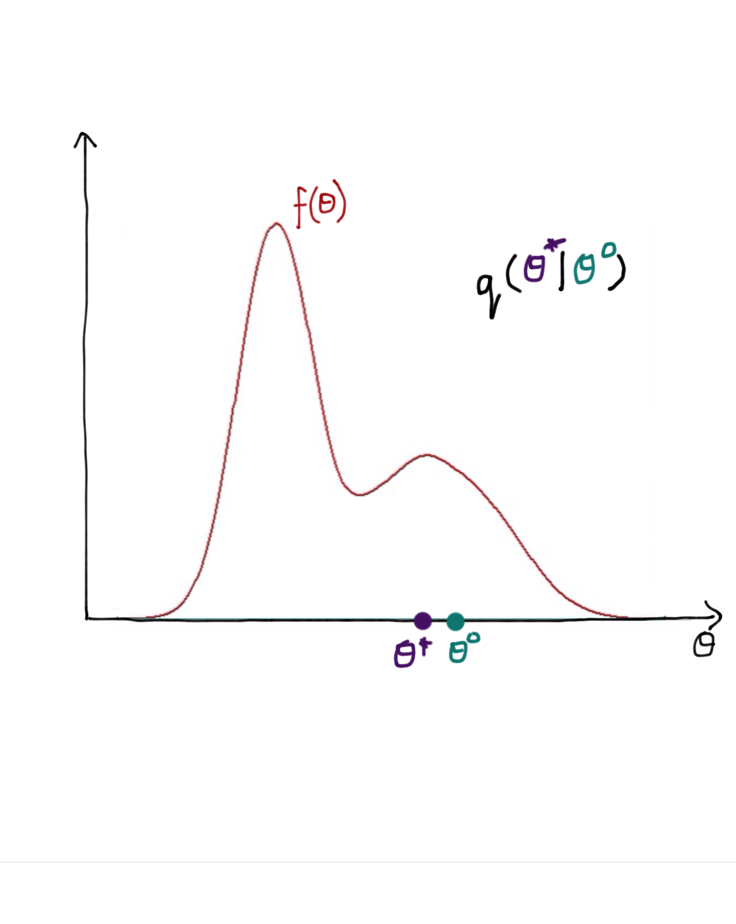
\includegraphics[width=0.8\linewidth]{MH2}

\column{.5\textwidth}
The algorithm proceeds as follows:\\
\begin{itemize}
\item Initialise $\theta^{0}$
\item Sample $\theta^* \sim q(\theta^*|\theta^{0})$
\item Compute acceptance probability, r
\item Draw $u \sim U(0,1)$;
\end{itemize}
\end{columns}
\end{frame}

\begin{frame}[label=sec-7-11]{Metropolis-Hastings}
\begin{columns}[c] 
\column{.5\textwidth} 
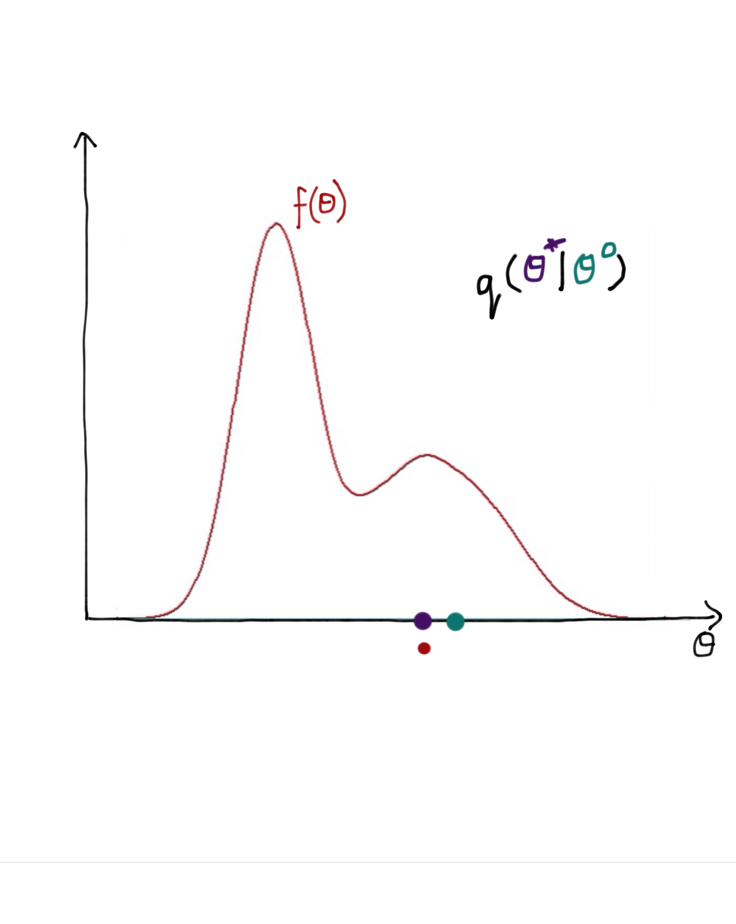
\includegraphics[width=0.8\linewidth]{MH5}

\column{.5\textwidth}
The algorithm proceeds as follows:\\
\begin{itemize}
\item Initialise $\theta^{0}$
\item Sample $\theta^* \sim q(\theta^*|\theta^{0})$
\item Compute acceptance probability, r
\item Draw $u \sim U(0,1)$;
\item Set new sample to 
\[
 \theta^{(s+1)} = 
\begin{cases}
    \theta^*, & \text{if } u < r\\
    \theta^{(s)}, & \text{if } u \geqslant r
\end{cases}
\]
\end{itemize}
\end{columns}
\end{frame}

\begin{frame}[label=sec-7-12]{Metropolis-Hastings}
\begin{columns}[c] 
\column{.5\textwidth} 
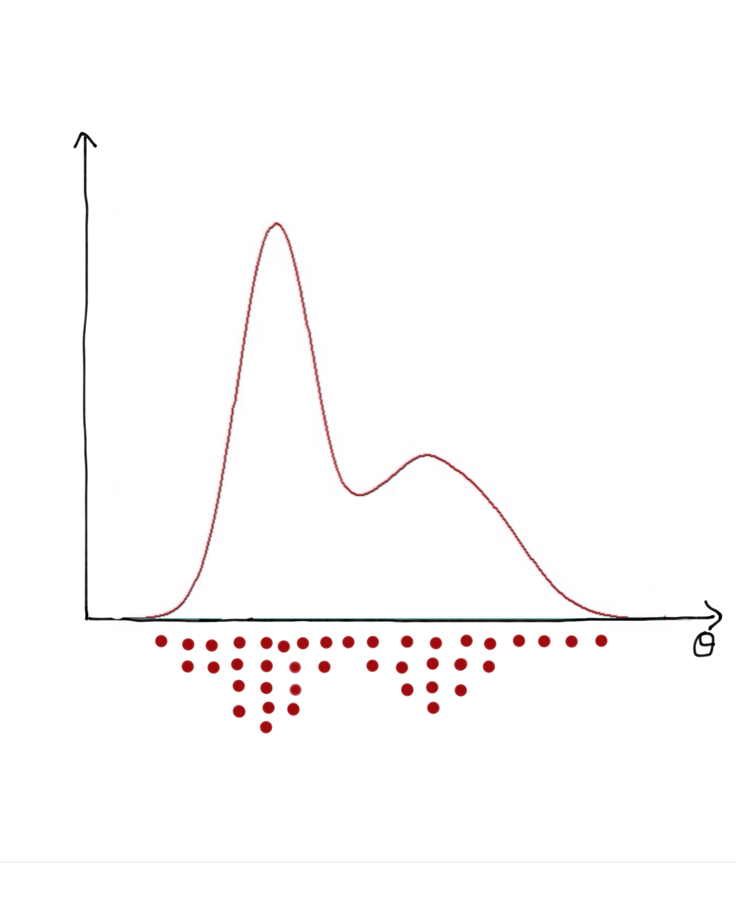
\includegraphics[width=0.8\linewidth]{MH6}

\column{.5\textwidth}
The algorithm proceeds as follows:\\
\begin{itemize}
\item Initialise $\theta^{0}$
\item Sample $\theta^* \sim q(\theta^*|\theta^{0})$
\item Compute acceptance probability, r
\item Draw $u \sim U(0,1)$;
\item Set new sample to 
\[
 \theta^{(s+1)} = 
\begin{cases}
    \theta^*, & \text{if } u < r\\
    \theta^{(s)}, & \text{if } u \geqslant r
\end{cases}
\]
\item Repeat
\end{itemize}
\end{columns}
\end{frame}

\section{MCMC in practice}
\label{sec-8}
\begin{frame}[label=sec-8-1]{Review}
In the practical you:
\begin{itemize}
\item used Metropolis-Hastings
\item with a Gaussian proposal distribution
\item to infer one parameter, $R_0$
\end{itemize} 
To infer more than one parameter we can use a multivariate Gaussian
\end{frame}

\begin{frame}[label=sec-8-2]{Multivariate Gaussian distribution}
\begin{columns}[c] 
\column{.5\textwidth} 
mean $\mu = \begin{bmatrix} 3 & 2 \end{bmatrix}$\\
covariance $\Sigma =  \begin{bmatrix} 25 & 0 \\ 0 & 9 \end{bmatrix}$
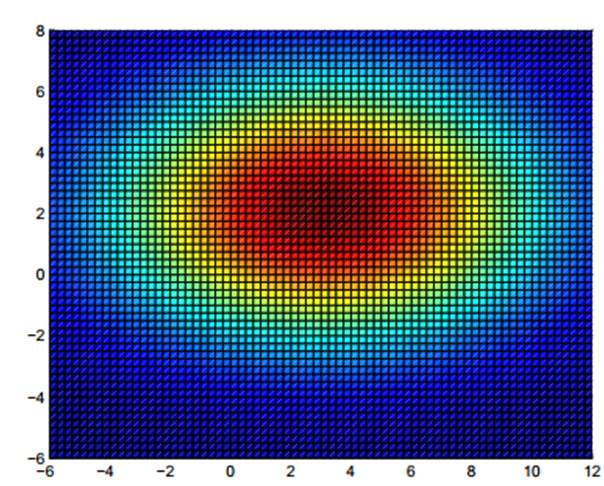
\includegraphics[width=0.8\linewidth]{MVN1}

\column{.5\textwidth}
mean $\mu = \begin{bmatrix} 3 & 2 \end{bmatrix}$\\
covariance $\Sigma =  \begin{bmatrix} 10 & 5 \\ 5 & 5 \end{bmatrix}$
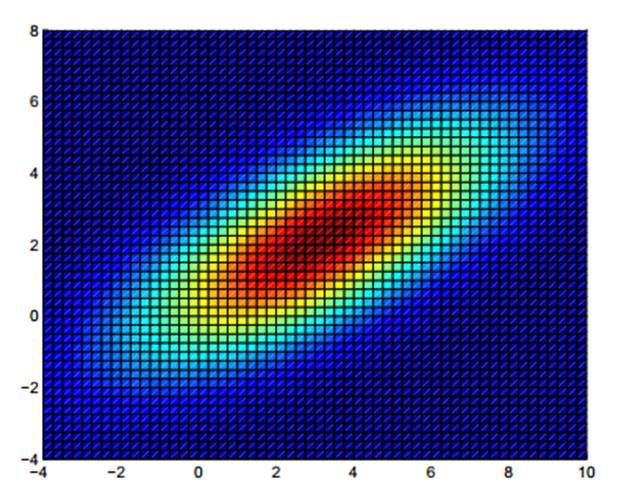
\includegraphics[width=0.8\linewidth]{MVN2}
\end{columns}  
\end{frame}

\begin{frame}[label=sec-8-3]{Choosing a proposal distribution}
For accurate and efficient MCMC we \alert{tune} the variance and covariance or the proposal distribution.\\~\\
\end{frame}

\begin{frame}[label=sec-8-4]{Choosing a proposal distribution}
If the variance term is too small, then the chain will never be able to move far enough from one mode to be able to identify the other.
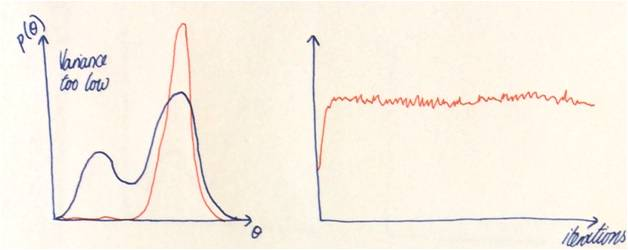
\includegraphics[width=1\linewidth]{Var1}
\end{frame}

\begin{frame}[label=sec-8-5]{Choosing a proposal distribution}
If the variance is too high, then many proposed values will be rejected and the chain will \textit{stick} in one place for many steps.
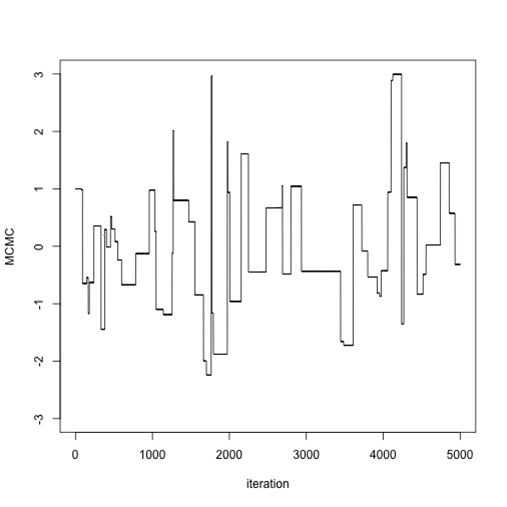
\includegraphics[width=1\linewidth]{Var2}
\end{frame}

\begin{frame}[label=sec-8-6]{Choosing a proposal distribution}
If the variance is just right, then the chain will efficiently explore the full shape of the target distribution.
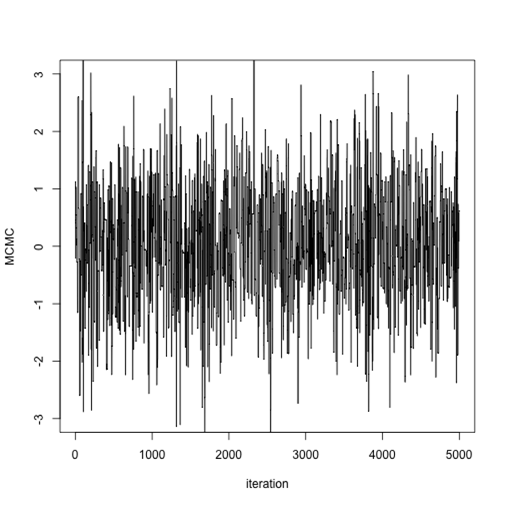
\includegraphics[width=1\linewidth]{Var3}
Try several different proposal distributions (\alert{pilot runs}), aiming for an acceptance rate between 24\%  and 40\%. 
\end{frame}

\begin{frame}[label=sec-8-7]{Adaptive MCMC}
\begin{itemize}
\item \alert{Adaptive MCMC} alters proposal distribution while chain is running. 
\item Start with large symmetric variance, scan around to find a mode. 
\item Then alter shape of proposal distribution to match covariance matrix of accepted values.
\item Eventually proposal density should match the shape of target density.
\end{itemize}
\end{frame}

\begin{frame}[label=sec-8-8]{Adaptive MCMC}
Two-stage adaptation
\begin{columns}[c] 
\column{.5\textwidth} 
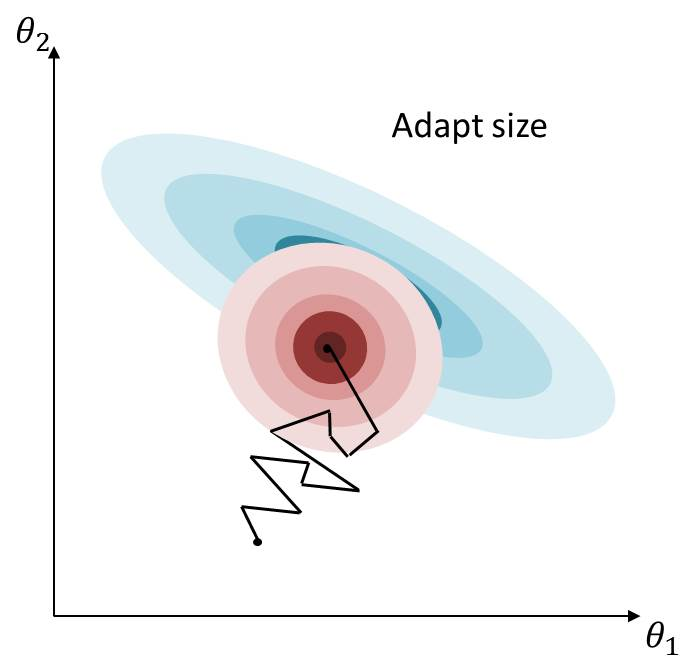
\includegraphics[width=.8\linewidth]{MH7.jpg}
\column{.5\textwidth} 
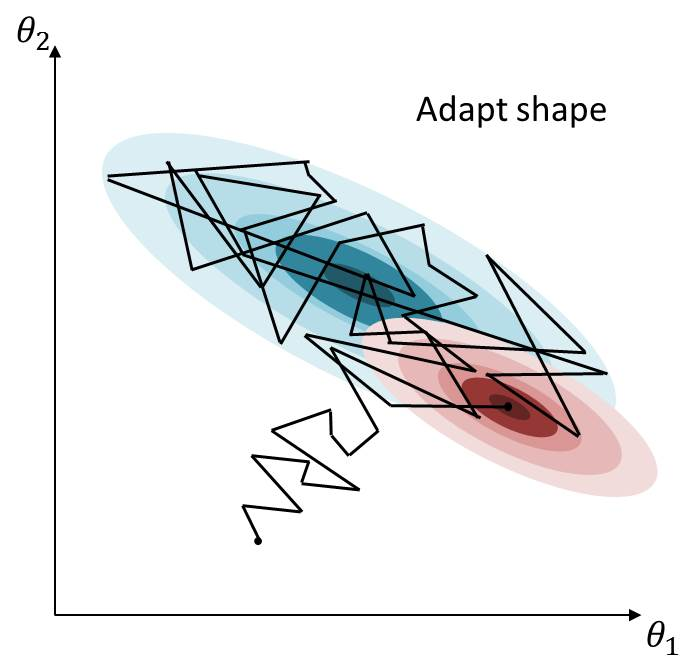
\includegraphics[width=.8\linewidth]{MH8.jpg}
\end{columns}
\end{frame}

\begin{frame}[label=sec-8-9]{Burn-in}
\begin{itemize}
\item We can start our MCMC chain anywhere.
\item It can take a while to reach and explore the target density $f(\theta)$.
\item Throw away early samples: \alert{burn-in} phase.
\item How much to discard?
\item Start several chains at different points. When their traces overlap, assume sampling from $f(\theta)$.
\end{itemize}
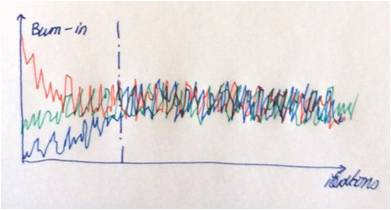
\includegraphics[width=.7\linewidth]{Burn}
\end{frame} 

\begin{frame}[label=sec-8-10]{MCMC sample size}
\begin{itemize}
\item In MCMC, each sample depends on the one before - \alert{auto-correlation}
\item Reduce degree of auto-correlation by \alert{thinning}, only retain every $n^{th}$ sample. 
\item Information content of MCMC samples is given by the \textbf{effective sample size (ESS)}
\item We use the R package \textit{tracer}.
\end{itemize}
\end{frame}

\begin{frame}[label=sec-8-11]{Advanced MCMC methods}
Lead in to tomorrow
\end{frame}


\end{document}